% Created 2021-03-22 Mon 13:05
% Intended LaTeX compiler: pdflatex

\documentclass[english]{article}
\usepackage[T1, T2A]{fontenc}
\usepackage[lutf8]{luainputenc}
\usepackage[english, russian]{babel}
\usepackage{minted}
\usepackage{graphicx}
\usepackage{longtable}
\usepackage{hyperref}
\usepackage{xcolor}
\usepackage{natbib}
\usepackage{amssymb}
\usepackage{stmaryrd}
\usepackage{amsmath}
\usepackage{caption}
\usepackage{mathtools}
\usepackage{amsthm}
\usepackage{tikz}
\usepackage{grffile}
\usepackage{extarrows}
\usepackage{wrapfig}
\usepackage{rotating}
\usepackage{placeins}
\usepackage[normalem]{ulem}
\usepackage{amsmath}
\usepackage{textcomp}
\usepackage{capt-of}

\usepackage{geometry}
\geometry{a4paper,left=2.5cm,top=2cm,right=2.5cm,bottom=2cm,marginparsep=7pt, marginparwidth=.6in}

 \usepackage{hyperref}
 \hypersetup{
     colorlinks=true,
     linkcolor=blue,
     filecolor=orange,
     citecolor=black,      
     urlcolor=cyan,
     }

\usetikzlibrary{decorations.markings}
\usetikzlibrary{cd}
\usetikzlibrary{patterns}
\usetikzlibrary{automata, arrows}

\newcommand\addtag{\refstepcounter{equation}\tag{\theequation}}
\newcommand{\eqrefoffset}[1]{\addtocounter{equation}{-#1}(\arabic{equation}\addtocounter{equation}{#1})}


\newcommand{\R}{\mathbb{R}}
\renewcommand{\C}{\mathbb{C}}
\newcommand{\N}{\mathbb{N}}
\newcommand{\rank}{\text{rank}}
\newcommand{\const}{\text{const}}
\newcommand{\grad}{\text{grad}}

\theoremstyle{plain}
\newtheorem{axiom}{Аксиома}
\newtheorem{lemma}{Лемма}
\newtheorem{manuallemmainner}{Лемма}
\newenvironment{manuallemma}[1]{%
  \renewcommand\themanuallemmainner{#1}%
  \manuallemmainner
}{\endmanuallemmainner}

\theoremstyle{remark}
\newtheorem*{remark}{Примечание}
\newtheorem*{solution}{Решение}
\newtheorem{corollary}{Следствие}[theorem]
\newtheorem*{examp}{Пример}
\newtheorem*{observation}{Наблюдение}

\theoremstyle{definition}
\newtheorem{task}{Задача}
\newtheorem{theorem}{Теорема}[section]
\newtheorem*{definition}{Определение}
\newtheorem*{symb}{Обозначение}
\newtheorem{manualtheoreminner}{Теорема}
\newenvironment{manualtheorem}[1]{%
  \renewcommand\themanualtheoreminner{#1}%
  \manualtheoreminner
}{\endmanualtheoreminner}
\captionsetup{justification=centering,margin=2cm}
\newenvironment{colored}[1]{\color{#1}}{}

\tikzset{->-/.style={decoration={
  markings,
  mark=at position .5 with {\arrow{>}}},postaction={decorate}}}
\makeatletter
\newcommand*{\relrelbarsep}{.386ex}
\newcommand*{\relrelbar}{%
  \mathrel{%
    \mathpalette\@relrelbar\relrelbarsep
  }%
}
\newcommand*{\@relrelbar}[2]{%
  \raise#2\hbox to 0pt{$\m@th#1\relbar$\hss}%
  \lower#2\hbox{$\m@th#1\relbar$}%
}
\providecommand*{\rightrightarrowsfill@}{%
  \arrowfill@\relrelbar\relrelbar\rightrightarrows
}
\providecommand*{\leftleftarrowsfill@}{%
  \arrowfill@\leftleftarrows\relrelbar\relrelbar
}
\providecommand*{\xrightrightarrows}[2][]{%
  \ext@arrow 0359\rightrightarrowsfill@{#1}{#2}%
}
\providecommand*{\xleftleftarrows}[2][]{%
  \ext@arrow 3095\leftleftarrowsfill@{#1}{#2}%
}
\makeatother
\author{Ilya Yaroshevskiy}
\date{\today}
\title{Лекция 6}
\hypersetup{
 pdfauthor={Ilya Yaroshevskiy},
 pdftitle={Лекция 6},
 pdfkeywords={},
 pdfsubject={},
 pdfcreator={Emacs 28.0.50 (Org mode )}, 
 pdflang={English}}
\begin{document}

\maketitle
\tableofcontents

\newcommand{\X}{\chi}
\newcommand{\A}{\mathfrak{A}}
\newcommand{\B}{\mathfrak{B}}
\newcommand{\M}{\mathfrak{M}}

\section{Сферические координаты в \(R^m\)}
\label{sec:orgace79bb}
\begin{examp}
\-
\begin{itemize}
\item \(r, \varphi_1, \dots \varphi_{m - 1}\)
\item \(\R^m \supset \R^{m - 1} \supset \dots \supset \R^2\)
В кажои из очередных пространств \(\R^k\) фиксируем ортогональное к \(\R^{k - 1}\)

\item \(\varphi_1\) --- угол между \(\overline{e_1}\) и \(Ox \in [0, \pi]\)
\item \(\varphi_2\) --- угол между \(\overline{e_2}\) и \(P_{2_(e_2\ \dots\ e_m)} (x) \in [0, \pi]\)
\item \(\vdots\)
\item \(\varphi_{m - 1}\) --- просто полярный угол в \(\R^m\)
\end{itemize}
\begin{center}
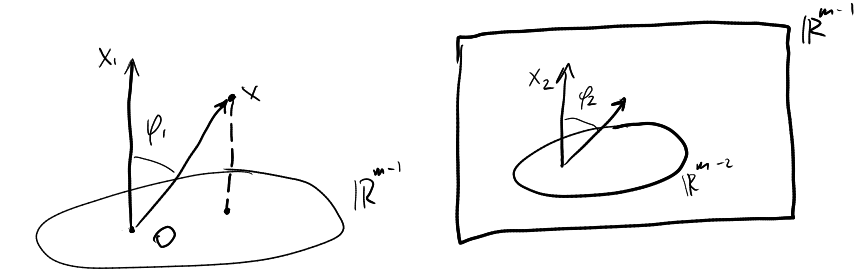
\includegraphics[scale=0.5]{6_1.png}
\end{center}
\[ x_1 = r\cos\varphi_1 \]
\[ x_2 = r \sin \varphi_1\cos\varphi_2 \]
\[ x_3 = 2 \sin \varphi_1 \sin\varphi_2 \cos\varphi_3 \]
\[ \vdots \]
\[ x_{m - 1} = r\sin\varphi_1 \dots \sin\varphi_{m - 2}\cos\varphi_{m - 1} \]
\[ x_m = r \sin\varphi_1 \dots \sin\varphi_{m - 2} \sin \varphi_{m - 1} \]
\[ J = r^{m - 1}\sin^{m - 2}\varphi_1\sin^{m - 3}\varphi_2 \dots \sin\varphi_{m - 2}\footnote{\text{В }\R^3\text{ ``географические`` координаты }J = r^2\cos\psi} \]
Сделаем в цикле эти координаты:
\begin{description}
\item[{шаг 1}] \(x_m = \rho_{m - 1}\sin\varphi_{m - 1}\) \\
\(x_{m - 1} = \rho_{m - 1}\cos\varphi_{m - 1}\) \\
\((x_1\ \dots\ x_n) \rightsquigarrow (x_1\ \dots\ x_{m - 2},\ \rho_{m - 1},\ \varphi_{m - 1})\)
\item[{шаг 2}] \(\rho_{m - 1} = \rho(m_2) \sin\varphi_{m - 2}\) \\
\(x_{m - 2} = \rho_{m - 2} \cos\varphi_{m - 2}\) \\
\((x_1\ \dots\ x_{m - 2},\ \rho_{m - 1},\ \varphi_{m -1}) \rightsquigarrow (x_1\ \dots\ x_{m - 3},\ \rho_{m - 2},\ \varphi_{m - 2},\ \varphi_{m - 1})\)
\item[{\(\vdots\)}] 

\item[{последний шаг}] \((x_1,\ \rho_2,\ \varphi_2\ \dots\ \varphi_{m - 1}) \rightsquigarrow (r,\ \varphi_1\ \dots\ \varphi_{m - 1})\) \\
\(\rho_2 = r\sin\varphi_1\) \\
\(x_1 = r \cos\varphi_1\)
\end{description}
\[ \lambda_m(\Omega) = \int\limits_\Omega 1 d\lambda_m \xlongequal[\text{1 шаг}]{} \int\limits_{\Omega_1} \rho_{m - 1} \xlongequal[\text{2 шаг}]{} \int\limits_{\Omega_2} \rho^2_{m - 2} \sin\varphi_{m - 2} \xlongequal[\text{3 шаг}]{} \int\limits_{\Omega_3} \rho^3_{m - 3} \sin^2\varphi_{m - 3}\sin\varphi_{m - 2} d\lambda = \]
\[ = \dots = \int\limits_{\Omega_{m - 1}}r^{m - 1}\sin^{n - 2}\varphi_{1} \dots \sin\varphi_{m - 2}\]
\end{examp}
\section{Произведение мер}
\label{sec:org6569904}
\begin{itemize}
\item \((X, \A, \mu)\)
\item \((Y, \B, \nu)\)
\end{itemize}
\begin{lemma}
\(\A, \B\) --- п/к \(\Rightarrow\) \(\A \times \B = \{A\times B \subset X \times Y | A \in \A,\ B\in\B\}\)
\end{lemma}
\begin{examp}
Ячейки: В \(\R^2 = \R^1 \times \R^1\ \A = \mathcal{P}^1,\ \B \in \mathcal{P}^1\) \\
\(A \times B\) --- ячейка из \(\mathcal{P}\)
\end{examp}
\begin{definition}
\(\mathcal{P} = \A \times \B\) --- множества из этой системы называются измеримыми прямоуг. \(m_o(A \times B) = \mu A\cdot \nu B\)
\end{definition}
\begin{theorem}
\-
\begin{enumerate}
\item \(m_0\) --- мера на \(\mathcal{P}\)
\item \(\nu,\mu\) --- \(\sigma\)-конечные \(\Rightarrow\) \(m_0\) --- тоже \(\sigma\)-конечная
\end{enumerate}
\end{theorem}
\begin{proof}
\-
\begin{enumerate}
\item ?\(m_0\) --- счетно аддитивна ?\(m_0 P = \sum m_o P_k\), если
\[ A \times B = P = \bigsqcup P_k\text{, где }P_k=A_k\times B_k \]
Наблюдение: \(\chi_{A \times B}(x, y) = \chi_A(x)\cdot\chi_B(y)\) \\
Тогда \(\chi_P = \sum \chi_{P_k}\), т.е.
\[ \forall x \in X, y \in Y\quad\chi_A(x)\chi_B(y) = \sum \chi_{A_k}(x)\chi_{B_k}(y) \]
проинтегрируем по \(y\) по мере \(\nu\):
\[ \chi_A(x) \nu B = \sum \chi_A(x)\cdot \nu B_k \]
Интегрируем по \(x\):
\[ \mu A \cdot \nu B - \sum \mu A_k \cdot \nu B_k  \]
\item Очев. \(\mu\) --- \(\sigma\)-конечная \(\Rightarrow\) \(X = \bigcup X_k\), \(\mu X_k\) --- конечная
\(nu\) --- \(\sigma\)-конечная \(\Rightarrow\) \(Y = \bigcup Y_n\), \(\nu Y_k\) --- конечная
\[ X \times Y = \bigcup X_k \timesy Y_n\quad m_0 \mu X_k \nu Y_n\text{ --- конечная} \]
\(\Rightarrow\) \(m_0\) --- \(\sigma\)-конечная мера
\end{enumerate}
\end{proof}
\begin{definition}
\-
\begin{itemize}
\item \((X, \A, \mu)\), \((Y, \B, \nu)\) --- пространства с мерой
\item \(\mu, \nu\) --- \(\sigma\)-конечные
\end{itemize}
Пусть \(m\) --- лебеговское продолжение меры \(m_0\) с п/к \(\A \times \B\) на \(\sigma\)-алгебра, которую будет обозначать \(\A \otimes \B\)
\end{definition}
\begin{definition}
\((X \times Y, \A \otimes \B, \nu \times \mu)\) --- произведение пространств с мерой \((X, \A, \mu)\) и \((Y, \B, \nu)\)
\end{definition}
\begin{remark}
\-
\begin{enumerate}
\item Это произведение ассоциативно
\item \(\sigma\)-конечность нужна для единственности произведения
\end{enumerate}
\end{remark}
\begin{theorem}
\(\lambda_m \times \lambda_n = \lambda_{n + m}\)
\end{theorem}
\begin{proof}
\color{red}Без доказательсва\color{black}
\end{proof}
\begin{definition}
\-
\begin{itemize}
\item \(X, Y\) --- множества
\item \(C \subset X \times Y\)
\end{itemize}
\[ C_x := \{y \in Y| (x, y) \in C\} \]
\[ C^y := \{x \in X| (x, y) \in C \} \]
\end{definition}
\begin{remark}
\[ \left(\bigcup\limits_\alpha C_\alpha\right)_x = \bigcup\left(C_\alpha\right)_x \]
\[ \left(\bigcap\limits_\alpha C_\alpha\right)_x = \bigcap\limits_\alpha\left(C_\alpha\right)_x \]
\[ \left(C \setminus C'\right)_x = C_x \setminus C'_x \]
\end{remark}
\begin{theorem}[Кавальери]
\-
\begin{itemize}
\item \((X, \A, \mu)\)
\item \((Y, \B, \nu)\)
\item \(\nu, \mu\) --- \(\sigma\)-конечные, полные
\item \(m := \mu \times \nu\)
\end{itemize}
Пусть \(C \in \A \otimes \B\) \\
\uline{Тогда}:
\begin{enumerate}
\item \(C_x \in \B\) при почти всех \(x\)
\item \(x \mapsto \nu(C_x)\) --- измеримая\footnote{функция задана при почти всех \(x\). Она равна почти везде некоторой измеримой функции, которая задана на всем \(X\). Это ``не мешает`` утверждению 3} функция на \(X\)
\item \(mC = \int\limits_X \nu(C_x)d\mu(x)\)
\end{enumerate}
Аналогичное верно для \(C^y\)
\end{theorem}
\begin{examp}
Половину шара сопоставляем с конусом.
\begin{center}
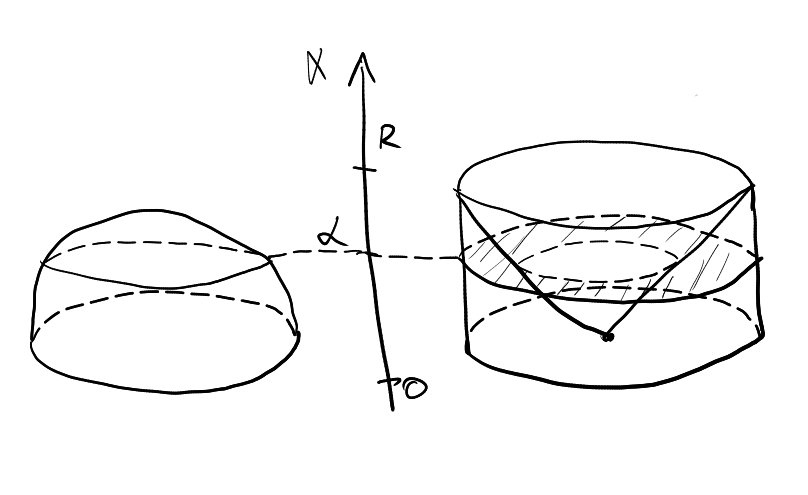
\includegraphics[scale=0.4]{6_2.png}
\end{center}
\begin{itemize}
\item \(C_x=\)круг
\item \(C_x=\)кольцо
\end{itemize}
\[ \lambda(C_x) = \pi(R^2 - x^2) \]
\[ \lambda(C_x) = \pi R^2 - \pi x^2 \]
\[ \nu(\frac{1}{2}\text{шара}) = \nu(\text{цилиндр}-\text{конус}) = \pi R^2 - \frac{1}{3} \pi R^2 = \frac{2}{3} \pi R^ \]
\end{examp}
\begin{proof}
\(\mathcal{D}\) --- система множеств, для которых выполнено 1. - 3. 
\begin{enumerate}
\item \(C = A\times B \Rightarrow C \in \mathcal{D}\)
\begin{enumerate}
\item \(C_x = \left[\begin{matrix} \emptyset & x \not\in A \\ B & x \in A\end{matrix}\right.\)
\item \(x \mapsto \nu(x)\) --- это функция \(\nu B \cdot \chi_A\)
\item \(\int \nu(C_x) d\mu = \int\limits_X \nu B \cdot \chi_A d\mu = \nu B \cdot \mu A = mC\)
\end{enumerate}
\item \(E_i \in D\), dis \(\Rightarrow\) \(\bigsqcup E_i \in D\) \\
\(E_i \in D \Rightarrow (E_i)_X\) --- измеримое почти везде \(\Rightarrow\) при почти всех \(x\) все \((E_i)_X\) -- измеримое \\
\begin{enumerate}
\item Тогда при этих \(x\ E_X = \bigsqcup(E_i)_X \in \B\)
\item \(\nu E_X = \sum \underbrace{\nu(E_i)_X}_\text{измеримая функция}\) \(\Rightarrow\) функция \(x \mapsto \nu E_X\) измеримая\(\footnotemark[\value{footnote}]\)
\item \[ \int\limits_X \nu E_X d\mu = \sum_i \int\limits_X \nu(E_i)_X = \sum_i mE_i = mE \]
\end{enumerate}
\item \(E_i \in \mathcal{D},\ E_1 \supset E_2 \supset \dots,\ E = \bigcap\limits_iE_i,\ \mu E_i < + \infty\) Тогда \(E \in \mathcal{D}\)
\[ \int\limits_X \nu(E_i)_X d\mu = mE_i < +\infty \Rightarrow \nu(E_i)_X\text{ --- конечная при почти всех }x \]
\begin{enumerate}
\item \(\forall x\) верно \((E_1)_X \supset (E_2)_X \supset \dots ,\ E_X = \bigcap (E_i)_X\). Тогда \(E_X\) --- измеримое при почти всех \(x\) и \(\lim\limits_{i \to + \infty} \nu(E_i)_X = \nu E_X\) при почти всех \(x\)
\item Таким образом \(x \mapsto \nu E_X\) --- измеримая\(\footnotemark[\value{footnote}]\)
\item \[ \int\limits_X \nu E_X d\mu = \lim \int \nu(E_i)_X d\mu = \lim mE_i = mE \]
Первое равенство по теореме Лебега о предельном переходе под знаком интеграла: \(|\nu (E_i)_X| \le \nu (E_1)_X\) --- из\(\footnotemark[\value{footnote}]\)
\end{enumerate}
\end{enumerate}
Итог: \(A_{ij} \in \mathcal{P} = \A \times \B\), то \(\color{red}??\color{black}\bigcup A_{ij} \in \mathcal{D}\)
\begin{enumerate}
\setcounter{enumi}{3}
\item \(mE = 0 \Rightarrow E \in \mathcal{D}\)
\[ mE = \inf\{\sum m_0 P_k | E \subset \bigcup P_k,\ P_k \in \mathcal{P}\} \]
--- теорема о лебеговском продолжении. \\
\(\exists\) множества \(H\) вида \(\bigcap\limits_e\bigsqcup\limits_X P_{ke}\) (т.е. \(H \in \mathcal{D}\)) \\
\(E \subset H, mH = mE = 0\)
\[ 0 = mH = \int\limits_X \nu H_x d\mu \Rightarrow \nu H_X \sim 0\text{ (\(=0\) при почти всех \(x\))} \]
\(E_X \subset H_x, \nu\) --- полная \(\Rightarrow\)
\begin{enumerate}
\item \(E_X\) --- измерима при почти всех \(x\)
\item \(\nu E_X = 0\) почти везде
\item \(\int \nu E_X d\mu = 0 = m E\)
\end{enumerate}
\item \(C\) --- \(m\)-измеримо, \(mC < + \infty\) тогда \(C \in \mathcal{D}\) \\
\(C = H \setminus e\), где \(H\) --- вида \(\color{red}???\color{black}\bigcup P_{ke},\ me = 0,\ mC = mH\)
\begin{enumerate}
\item \(C_x = H_x \setminus e_X\) --- измерима при почти всех \(x\), т.к. \(\nu\) --- полная
\item \(\nu e_X = 0\) при почти всех \(x\) \(\Rightarrow\) \(\nu C_x = \nu H_x - \nu e_X = \nu H_X\) \(\Rightarrow\) измерима
\item \(\int\limits_X \nu C_x d\mu = \int\limits_X \nu H_x d\mu = mH = mC\)
\end{enumerate}
\item \(C\) --- произвольное измеримое множество в \(X \times Y\) \(\Rightarrow\) \(C \in \mathcal{D}\) \\
\[ X = \bigsqcup X_k,\ \mu X_k < + \infty,\ Y = \bigsqcup Y_j,\ \nu Y_j < + \infty \]
\[ C = \bigsqcup (C \cap (X_k \times Y_j))\text{ --- используем 2.}\]
\end{enumerate}
\end{proof}
\begin{corollary}
\(C\) --- измеримое в \(X\times Y\). Пусть \(P_q(C) = \{x \in X| C_x \neq 0\}\) --- проекция \(C\) на \(X\). Если \(P_1(C)\) --- измеримое, то:
\[ mC = \int\limits_{P_1(C)} \nu(C_x) d\mu \]
\end{corollary}
\begin{proof}
при \(x \not\in P_1(C)\ \nu(C_x) = 0\)
\end{proof}
\begin{remark}
\-
\begin{enumerate}
\item \(С\) --- измеримое \(\not\Rightarrow\) \(P_1(C)\) --- измеримое
\item \(C\) --- измеримое \(\not\Rightarrow\) \(\forall x\ C_x\) --- измеримо
\item \(\forall x\forall y\ C_x,C^y\) --- измеримые \(\not\Rightarrow\) \(C\) --- измеримое (пример Серпинского)
\end{enumerate}
\end{remark}
\end{document}
